\documentclass{article}
\usepackage[utf8]{inputenc}
\usepackage{graphicx}
\usepackage{etoolbox}
\graphicspath{ {Graphics/} }
\AtBeginEnvironment{quote}{\singlespacing\small}

\title{Solar Panel Investigation \\ Practice Assessment}
\author{Thomas Bass}
\begin{document}

\maketitle


\part{The Plan}

\section{Working Title}
\begin{quote}
the working title of the investigation
\end{quote}
The Physics of Solar Panels

\section{Aim}
\begin{quote}
the aim of the investigation
\end{quote}
This investigation will
\begin{enumerate}
  \item Investigate the proportionality of light intensity and voltage
  \item Investigate the proportionality of light intensity and current
  \item Deduce the resistance of the solar panel
  \item Investigate the effect of light colour and voltage
\end{enumerate}

\section{Initial Experiments}
\begin{quote}
an outline of the initial experiments
\end{quote}
For ease of recording, we want the apparatus to return values that can be accurately and quickly recorded. This means we want the equiptment to return values between 0 and 999, and no more than two decimal places
\begin{itemize}
  \item Find an appropriate initial intensity
  \begin{itemize}
    \item First, the LCD panel was connected to power and turned on
    \item Then, the panel was set to maximim brightness, and the light meter attached
    \item The light meter was then set to 2000, as that gave integer values between 0 and 999
  \end{itemize}
  \item Find appropriate voltmeter sensitivity settings
  \begin{itemize}
    \item With the panel still turned on, the solar cell was affixed to the LCD panel, using blue tack to minimise light leak
    \item Then, the panel was set to maximum brightness, and the solar cell was connected to the Multimeter
    \item The multimeter was adjusted to 200m for voltage, as this sensitivity returned values between 0 and 999, and no more than two decimal places
  \end{itemize}
  \item Find appropriate ammeter sensitivity settings
  \begin{itemize}
    \item The multimeter was then set to 20$\mu$ for current, as this sensitivity returned values between 0 and 999, and no more than two decimal places
  \end{itemize}
\end{itemize}
\subsection{Initial Experiment Results}
\begin{table}[!ht]
\centering
\caption{Initial Experiment Results}
\label{Initial Experiment Results}
\begin{tabular}{|l|l|l|l|l|}
\hline
\textbf{Brightness}      & \textbf{Light Level} & \textbf{Ambient}   & \textbf{Potential Difference} & \textbf{Current}        \\ \hline
\textit{{[}arbitrary{]}} & \textit{{[}Lux{]}}   & \textit{{[}Lux{]}} & \textit{{[}Millivolt{]}}      & \textit{{[}Microamp{]}} \\ \hline
16                       & 248                  & 22                 & 45.2                          & 4.4                     \\ \hline
0                        & 1                    & 23                 & 0                             & 0                       \\ \hline
\end{tabular}
\end{table}
These results show that the sensitivity settings are correct, as the maximum results are within the range of the multimeter, and give results to a suitable decimal place.


\section{Apparatus}
\begin{quote}
a list of the required apparatus
\end{quote}
\begin{enumerate}
  \item Solar Cell
  \item RGB LCD Panel
  \item Blue tack
  \item Crocodile clips and cables
  \item Multimeter
  \item Light Meter
\end{enumerate}

\section{Initial Diagram}
\begin{quote}
a diagram of the initial experiment
\end{quote}
\section{Risk Assessment}
\begin{quote}
a risk assessment
\end{quote}

\section{Timeline}
\begin{quote}
a rough breakdown of how the two-week period of intensive practical work will be spent
\end{quote}
\pagebreak [4]
\part{The Report}

\section{Aim}
\begin{quote}
  a statement of aim
\end{quote}
This investigation will
\begin{enumerate}
  \item Investigate the proportionality of light intensity and voltage
  \item Investigate the proportionality of light intensity and current
  \item Deduce the resistance of the solar panel
  \item Investigate the effect of light colour and voltage
\end{enumerate}

\section{Results}

\begin{table}[!ht]
\centering
\caption{Measuring change in Potential Difference and Current with change in Light Level}
\label{my-label}
\begin{tabular}{|l|l|l|l|l|l|l|l|l|}
\hline
\textbf{Brightness}      & \textbf{Light Level} & \textbf{Ambient}   & \multicolumn{3}{l|}{\textbf{Potential Difference}} & \multicolumn{3}{l|}{\textbf{Current}}        \\ \hline
\textit{{[}arbitrary{]}} & \textit{{[}Lux{]}}   & \textit{{[}Lux{]}} & \multicolumn{3}{l|}{\textit{{[}Millivolt{]}}}      & \multicolumn{3}{l|}{\textit{{[}Microamp{]}}} \\ \hline
16                       & 248                  & 22                 & 45.2            & 44.7            & 44.9           & 4.4            & 4.43         & 4.32         \\ \hline
15                       & 205                  & 23                 & 38              & 38.1            & 38.1           & 3.69           & 3.71         & 3.71         \\ \hline
14                       & 169                  & 21                 & 31.7            & 31.7            & 31.6           & 3.08           & 3.08         & 3            \\ \hline
13                       & 139                  & 22                 & 26.2            & 26.3            & 26.6           & 2.54           & 2.55         & 2.56         \\ \hline
12                       & 114                  & 23                 & 21.5            & 21.5            & 21.4           & 2.08           & 2.08         & 2.09         \\ \hline
11                       & 91                   & 23                 & 17.4            & 17.1            & 17.2           & 1.69           & 1.73         & 1.72         \\ \hline
10                       & 74                   & 22                 & 14.1            & 13.6            & 14             & 1.37           & 1.3          & 1.37         \\ \hline
9                        & 58                   & 21                 & 11.2            & 11.3            & 11.1           & 1.08           & 1.08         & 1.06         \\ \hline
8                        & 46                   & 21                 & 8.8             & 8.8             & 8.7            & 0.86           & 0.87         & 0.87         \\ \hline
7                        & 34                   & 22                 & 6.8             & 6.9             & 7              & 0.66           & 0.66         & 0.65         \\ \hline
6                        & 25                   & 22                 & 5.1             & 5.1             & 5.2            & 0.5            & 0.54         & 0.54         \\ \hline
5                        & 19                   & 23                 & 3.9             & 3.7             & 3              & 0.38           & 0.36         & 0.3          \\ \hline
4                        & 13                   & 24                 & 2.8             & 2.8             & 2.7            & 0.27           & 0.3          & 0.28         \\ \hline
3                        & 9                    & 21                 & 2               & 1.9             & 1.9            & 0.19           & 0.2          & 0.19         \\ \hline
2                        & 5                    & 22                 & 1.3             & 1.3             & 1.4            & 0.12           & 0.12         & 0.11         \\ \hline
1                        & 2                    & 23                 & 0.7             & 0.7             & 0.6            & 0.07           & 0.07         & 0.07         \\ \hline
0                        & 1                    & 23                 & 0               & 0               & 0              & 0              & 0            & 0            \\ \hline
\end{tabular}
\end{table}

\begin{table}[!ht]
\centering
\caption{Measuring change in Potential Difference with change in Wavelength}
\label{my-label}
\begin{tabular}{|l|l|l|l|}
\hline
\textbf{Wavelength}       & \textbf{Brightness} & \textbf{Current}        & \textbf{Potential Difference} \\ \hline
\textit{{[}nanometers{]}} & \textit{{[}lux{]}}  & \textit{{[}microamp{]}} & \textit{{[}millivolt{]}}      \\ \hline
400                       & 34                  & 0.88                    & 9                             \\ \hline
425                       & 50                  & 1.2                     & 12.3                          \\ \hline
450                       & 55                  & 1.18                    & 12.1                          \\ \hline
475                       & 120                 & 2.04                    & 21                            \\ \hline
500                       & 155                 & 2.22                    & 22.8                          \\ \hline
525                       & 149                 & 2.04                    & 21                            \\ \hline
550                       & 166                 & 2.51                    & 25.7                          \\ \hline
575                       & 194                 & 3.26                    & 33.4                          \\ \hline
600                       & 130                 & 2.56                    & 26.3                          \\ \hline
625                       & 75                  & 1.62                    & 16.7                          \\ \hline
650                       & 60                  & 1.62                    & 16.7                          \\ \hline
675                       & 60                  & 1.62                    & 16.7                          \\ \hline
700                       & 60                  & 1.62                    & 16.7                          \\ \hline
725                       & 40                  & 1.06                    & 10.9                          \\ \hline
750                       & 21                  & 0.61                    & 6.3                           \\ \hline
775                       & 9                   & 0.29                    & 3                             \\ \hline
\end{tabular}
\end{table}
\section{Data Processing}
\text{These results can be plotted as line graphs. First, I plotted Brightness against Light Level from Table 2, to see if the linear unit increase of Brightness corresponds to a linear incrase in light level \\}
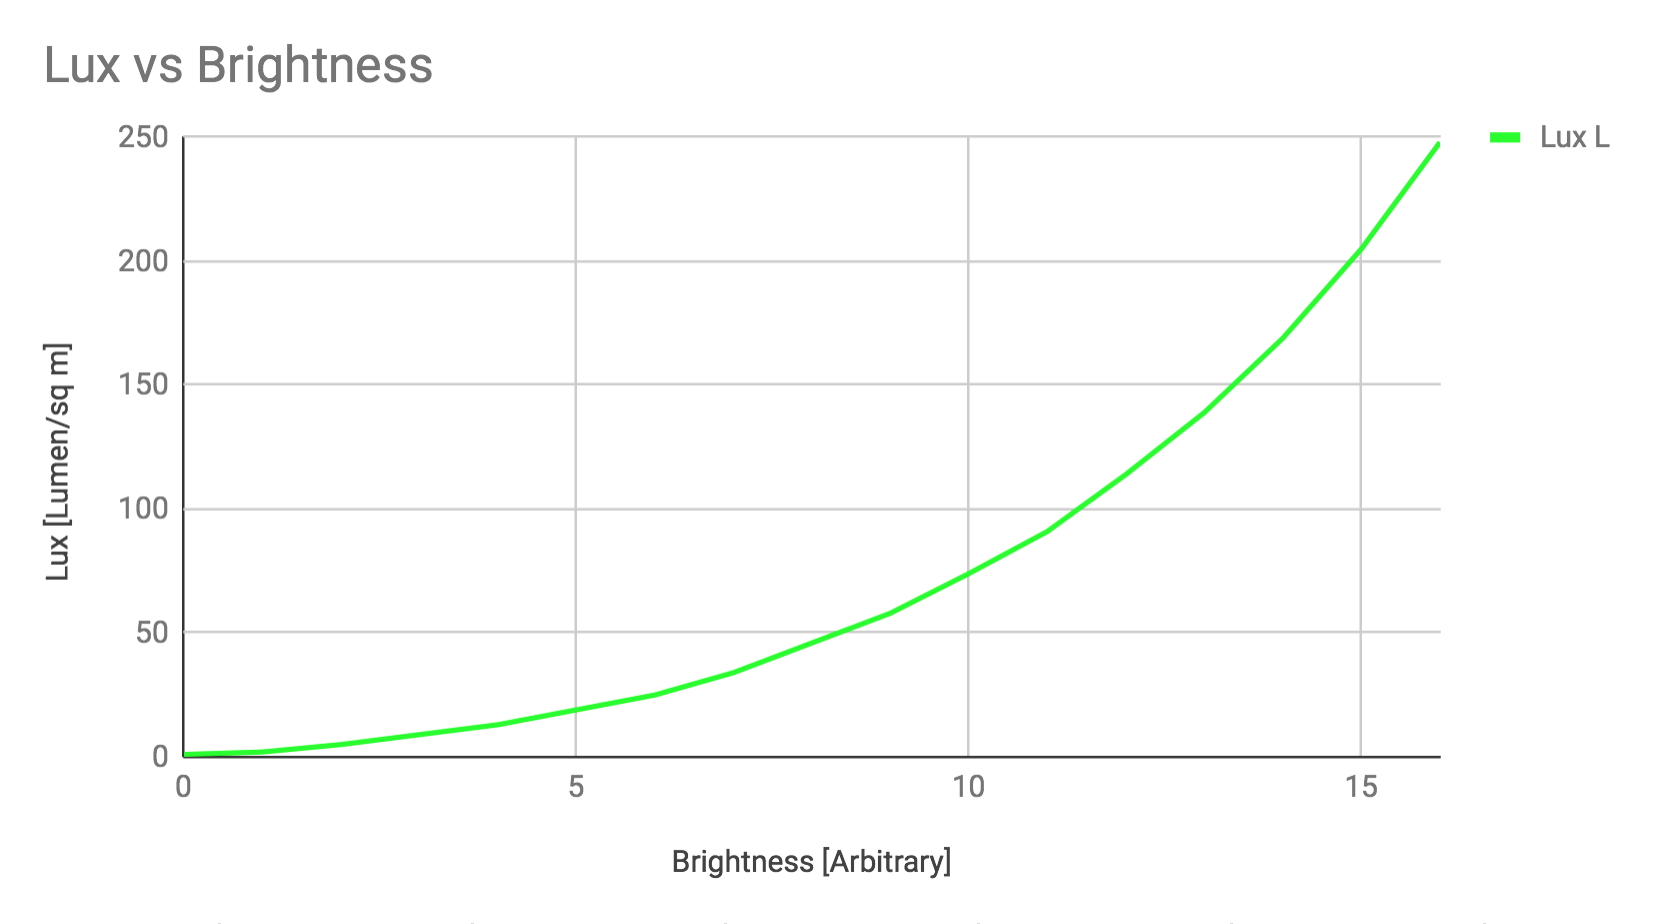
\includegraphics[scale=0.4]{Lux_v_Brightness.jpg}
\text{Then, as we have multiple results, I processed them to generate averages, ranges, and error bars}

% Please add the following required packages to your document preamble:

\begin{table}[]
\centering
\caption{Processed data showing the averages and errors}
\label{my-label}
\begin{tabular}{|l|l|l|l|l|l|l|l|l|}
\hline
\multirow{}{}{\textbf{\begin{tabular}[c]{@{}l@{}}Light\\ level\end{tabular}}} & \textbf{PD}           & \textbf{CUR}          & \textbf{PD}           & \textbf{CUR}          & \textbf{PD}           & \textbf{PD}           & \textbf{CUR}          & \textbf{CUR}          \\ \cline{2-9}
                                                                                & \textit{\textbf{Avg}} & \textit{\textbf{Avg}} & \textit{\textbf{Ran}} & \textit{\textbf{Ran}} & \textit{\textbf{Max}} & \textit{\textbf{Min}} & \textit{\textbf{Max}} & \textit{\textbf{Min}} \\ \hline
248                                                                             & 44.93                 & 4.38                  & 0.5                   & 0.11                  & 45.18                 & 44.68                 & 4.44                  & 4.33                  \\ \hline
205                                                                             & 38.07                 & 3.7                   & 0.1                   & 0.02                  & 38.12                 & 38.02                 & 3.71                  & 3.69                  \\ \hline
169                                                                             & 31.67                 & 3.05                  & 0.1                   & 0.08                  & 31.72                 & 31.62                 & 3.09                  & 3.01                  \\ \hline
139                                                                             & 26.37                 & 2.55                  & 0.4                   & 0.02                  & 26.57                 & 26.17                 & 2.56                  & 2.54                  \\ \hline
114                                                                             & 21.47                 & 2.08                  & 0.1                   & 0.01                  & 21.52                 & 21.42                 & 2.09                  & 2.08                  \\ \hline
91                                                                              & 17.23                 & 1.71                  & 0.3                   & 0.04                  & 17.38                 & 17.08                 & 1.73                  & 1.69                  \\ \hline
74                                                                              & 13.9                  & 1.35                  & 0.5                   & 0.07                  & 14.15                 & 13.65                 & 1.39                  & 1.32                  \\ \hline
58                                                                              & 11.2                  & 1.07                  & 0.2                   & 0.02                  & 11.3                  & 11.1                  & 1.08                  & 1.06                  \\ \hline
46                                                                              & 8.77                  & 0.87                  & 0.1                   & 0.01                  & 8.82                  & 8.72                  & 0.88                  & 0.87                  \\ \hline
34                                                                              & 6.9                   & 0.66                  & 0.2                   & 0.01                  & 7                     & 6.8                   & 0.67                  & 0.66                  \\ \hline
25                                                                              & 5.13                  & 0.53                  & 0.1                   & 0.04                  & 5.18                  & 5.08                  & 0.55                  & 0.51                  \\ \hline
19                                                                              & 3.53                  & 0.35                  & 0.9                   & 0.08                  & 3.98                  & 3.08                  & 0.39                  & 0.31                  \\ \hline
13                                                                              & 2.77                  & 0.28                  & 0.1                   & 0.03                  & 2.82                  & 2.72                  & 0.3                   & 0.27                  \\ \hline
9                                                                               & 1.93                  & 0.19                  & 0.1                   & 0.01                  & 1.98                  & 1.88                  & 0.2                   & 0.19                  \\ \hline
5                                                                               & 1.33                  & 0.12                  & 0.1                   & 0.01                  & 1.38                  & 1.28                  & 0.13                  & 0.12                  \\ \hline
2                                                                               & 0.67                  & 0.07                  & 0.1                   & 0                     & 0.72                  & 0.62                  & 0.07                  & 0.07                  \\ \hline
1                                                                               & 0                     & 0                     & 0                     & 0                     & 0                     & 0                     & 0                     & 0                     \\ \hline
\end{tabular}
\end{table}

\section{Summary}
\begin{quote}
  a word-processed summary of approximately 300 words written after completing the project, including an outline of any changes from the original plan
\end{quote}












\end{document}
